\documentclass[preview]{standalone}

\usepackage[english]{babel}
\usepackage{amsmath}
\usepackage{amssymb}
\usepackage{tikz}
\usepackage{verbatim}
\usepackage{nicematrix}
\usepackage{fancyvrb}
\usepackage[hyphens]{url}

\usepackage{xcolor}
\usepackage{color}
\usepackage{colortbl}
\usepackage{xspace} % fix missing spaces after fancy commands e.g. \dagster
\usepackage{makecell}
\usepackage{fancyvrb}
\usepackage{tikz}
\usepackage{tikzscale}
\usepackage{pgfplots}
\usepackage{graphicx}
\usepackage{todonotes}
\usepackage{wrapfig}
%\usepackage{dingbat}
% to be able to draw some self-contained figs
\usepackage{tikz}
\usepackage{amsmath}
\usepackage{subcaption}
\usepackage[misc]{ifsym}
\usepackage{nicematrix}



\newcommand{\dagster}{\textsc{Dagster}\xspace}
\newcommand{\tinisat}{\textsc{TiniSAT}\xspace}
\newcommand{\lingeling}{\textsc{Lingeling}\xspace}
\newcommand{\gnoveltyp}{\textsc{gNovelty$+$}\xspace}
\newcommand{\modezero}{C\xspace}
\newcommand{\modeone}{CL\xspace}
\newcommand{\modetwo}{CS\xspace}
\newcommand{\modethree}{CSL\xspace}




\begin{document}

\begin{center}


\begin{figure*}[]
        \centering
		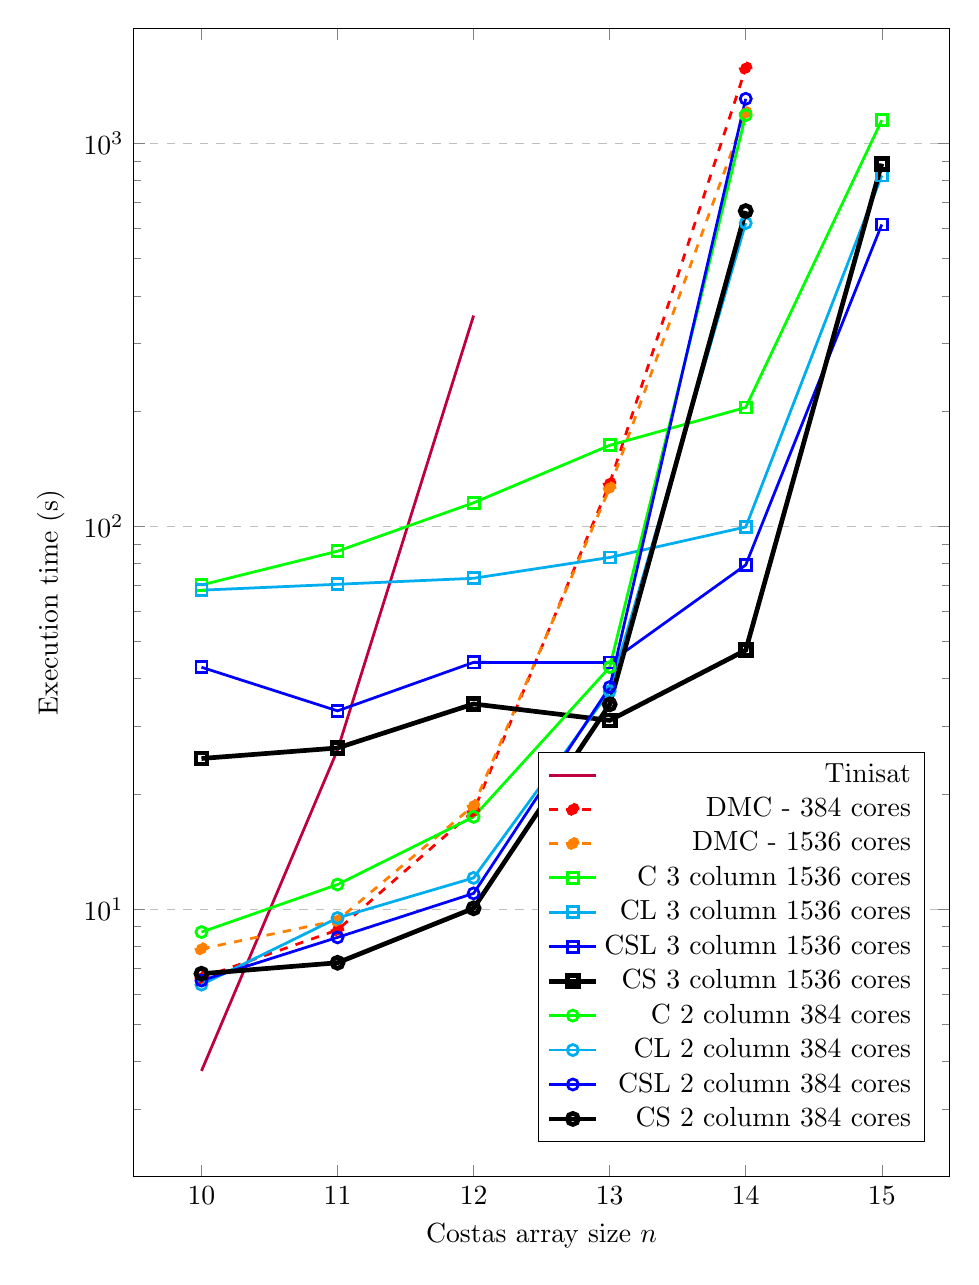
\begin{tikzpicture}
		\begin{axis}[
			title={},
			xlabel={Costas array size $n$},
			ylabel={Execution time (s)},
			%xmin=0, xmax=0.25,
			ymin=2.00, ymax=2000.00,
			ymode=log,
			xtick={10,11,12,13,14,15},
			%ytick={0,20,40,60,80,100},
			%yticklabel=$\pgfmathprintnumber{\tick}\%$,
			legend pos=south east,
			legend cell align=right,
			ymajorgrids=true,
			grid style=dashed,
			xticklabel style={/pgf/number format/fixed},
			width = 340,
			height = 460
		]




\addplot[color=purple,line width=1.0pt] coordinates {
(10,3.7782273292541504)(11,26.04908299446106)(12,355.1301419734955)}node[pos=0.8](endofplotsquare){} ;
\addlegendentry{Tinisat}




%\addplot[mark = diamond,color=green,line %width=1.0pt,dashed] coordinates {
%(10, 2.4890098571777344)
%(11, 15.25694990158081)
%(12, 149.58365178108215)
%(13, 2073.277750492096)
%(14, 3001.0201098918915)
%(15, 3001.0185282230377)
%(16, 3001.017208814621)
%(17, 3001.0177602767944)
%}node[pos=0.8](endofplotsquare){} ;
%\addlegendentry{DMC - laptop}


\addplot[mark = *,color=red,line width=1.0pt,dashed] coordinates {
(10, 6.614523410797119)
(11, 8.821394920349121)
(12, 18.032766580581665)
(13, 129.34079885482788)
(14, 1572.7557713985443)
%(15, 3004.0578289031982)
}node[pos=0.8](endofplotsquare){} ;
\addlegendentry{DMC - 384 cores}


\addplot[mark = *,color=orange,line width=1.0pt,dashed] coordinates {
(10, 7.872957944869995)
(11, 9.344036340713501)
(12, 18.633763074874878)
(13, 125.84372735023499)
(14, 1201.838926076889)
}node[pos=0.8](endofplotsquare){} ;
\addlegendentry{DMC - 1536 cores}






%\addplot[color=black,line width=0.8pt,dotted] coordinates {
%(10,268.601)
%(11,409.919)
%(12,612.876)
%(13,965.892)
%(14,1624.668)
%}node[pos=0.8](endofplotsquare){} ;
%\addlegendentry{\modezero 4 column 1536 cores}


\addplot[mark = square,color=green,line width=1.0pt] coordinates {
(10,70.254)
(11,86.081)
(12,115.172)
(13,162.719)
(14,204.369)
(15,1150.111)
}node[pos=0.8](endofplotsquare){} ;
\addlegendentry{\modezero 3 column 1536 cores}

\addplot[mark = square,color=cyan,line width=1.0pt] coordinates {
(10,68.087)
(11,70.551)
(12,73.140)
(13,82.886)
(14,99.570)
(15,824.921)
}node[pos=0.8](endofplotsquare){} ;
\addlegendentry{\modeone 3 column 1536 cores}


\addplot[mark = square,color=blue,line width=1.0pt] coordinates {
(10,42.836)
(11,32.946)
(12,44.104)
(13,44.056)
(14,79.275)
(15,614.229)
}node[pos=0.8](endofplotsquare){} ;
\addlegendentry{\modethree 3 column 1536 cores}

\addplot[mark = square,color=black,line width=1.7pt] coordinates {
(10,24.741)
(11,26.357)
(12,34.344)
(13,31.114)
(14,47.458)
(15,885.323)
}node[pos=0.8](endofplotsquare){} ;
\addlegendentry{\modetwo 3 column 1536 cores}





\addplot[mark = o,color=green,line width=1.0pt] coordinates {
(10,8.709)(11,11.592)(12,17.416)(13,42.837)(14,1185.395)
}node[pos=0.8](endofplotsquare){} ;
\addlegendentry{\modezero 2 column 384 cores}

\addplot[mark = o,color=cyan,line width=1.0pt] coordinates {
(10,6.349)(11,9.481)(12,12.062)(13,37.085)(14,619.429)
}node[pos=0.8](endofplotsquare){} ;
\addlegendentry{\modeone 2 column 384 cores}


\addplot[mark = o,color=blue,line width=1.0pt] coordinates {
(10,6.506)(11,8.435)(12,10.991)(13,38.013)(14,1308.012)
}node[pos=0.8](endofplotsquare){} ;
\addlegendentry{\modethree 2 column 384 cores}

\addplot[mark = o,color=black,line width=1.7pt] coordinates {
(10,6.779)(11,7.242)(12,10.048)(13,34.258)(14,665.972)
}node[pos=0.8](endofplotsquare){} ;
\addlegendentry{\modetwo 2 column 384 cores}




		\end{axis}
		\end{tikzpicture}
		%\vspace{-18pt}
		\caption{Runtime performance of \dagster\ against model counting with \tinisat\ and \textsc{DMC} on  Costas problems with different number of columns in the decomposition and processor cores. \modezero = CDCL only; \modeone = CDCL + local search; \modetwo = CDCL + strengthener; \modethree = CDCL + strengthener + local search}
    \end{figure*}



\end{center}

\end{document}
